\topictitle{Introduction to Visualisation - What, Why, How}{Topic 1}

\begin{topicsummary}
    \item We establish core definitions of data visualisation and clarify the difference between representation and presentation.
    \item We explain why visualisation matters by focusing on human judgement, visual perception, and external memory.
    \item We show why summary statistics are not enough by using Anscombe's Quartet and the Datasaurus example.
    \item We introduce Munzner's four-level framework and connect it to the three design questions: what, why, and how.
    \item We close with a concrete walkthrough of the what-why-how method using the Gapminder bubble chart.
\end{topicsummary}

\section{Defining Data Visualisation}

There is \textbf{no single, universally accepted definition} of data visualisation. A widely used working definition describes it as \textit{``the visual representation and presentation of data to facilitate understanding''} \parencite{kirk2019}. Here, \textbf{representation} refers to the transformation of data into visual marks and chart structures, whereas \textbf{presentation} concerns how those representations are situated through interaction, layout, annotation, and interface context.

\margincitebox[Definitions]{kirk2019,munzner2014}

Kirk's phrase ``facilitate understanding'' can be read as a three-step progression \parencite[p.~29]{kirk2019}. First, viewers \textbf{perceive}: they notice what is visible in the chart. Next, they \textbf{interpret}: they connect those visible elements to context. Finally, they \textbf{comprehend}: they decide what the information means for their own question or action.

To make this boundary clearer, Kirk also separates data visualisation from several adjacent terms \parencite[pp.~27--29]{kirk2019}:
\begin{itemize}
    \item \textbf{Infographics} usually focus on explanatory communication and often combine charts with illustration and text.
    \item \textbf{Information visualisation} is often used for abstract structures and relationships, such as trees and networks.
    \item \textbf{Information design} is a broader practice that includes many functional communication artefacts beyond charts.
    \item \textbf{Data art} primarily emphasises expression and aesthetics rather than analytical understanding.
    \item \textbf{Dashboards} are multi-view compositions, so they should not be treated as a single chart type.
    \item \textbf{Storytelling} requires narrative context; a chart alone does not automatically form a story.
\end{itemize}

\section{Why Visualisation Matters}
\label{sec:why-visualisation}
\noindent After clarifying what visualisation is, the next question is why we still need it when advanced algorithms are available. The key point is simple: visualisation does not replace computation. It complements computation by keeping human judgement in the analytical loop.

Munzner argued that \textit{``Computer-based visualization systems provide visual representations of datasets designed to help people carry out tasks more effectively.''} \parencite{munzner2014}. This means that visualisation is suitable when there is a need to augment human capabilities rather than replace people with computational decision-making methods.

\subsection*{The human in the loop}
Visualisation is especially valuable when tasks are ill-specified. In many real settings, analysts do not know the exact question in advance, and the question itself evolves as evidence appears. In this situation, fully automated pipelines are limited because they require precise objectives early. Visualisation supports iterative sensemaking by allowing people to form, test, and revise hypotheses while directly inspecting the data.

\marginnotebox{NOTE}{Generally it's better to have an image than a number. Humans are not good at interpreting numbers - Better to combine multi-dimensional information into a single, easily understandable form - Easier to extract and emphasise important info.}

\subsection*{Advantages of Visual Perception}
The visual system provides a high-bandwidth channel to the brain, so people can process many signals in parallel. In practice, this advantage comes from speed (gist recognition in about 20 milliseconds), parallel processing, and \textbf{pre-attentive} detection. Visualisations also act as \textbf{external memory}: analysts can offload details to a visual artefact and return later to compare patterns and hypotheses.

\subsection*{Where visualisation is used in practice}
Visualisation supports more than one task stage. In task terms, we often describe this as \textbf{discover--design--communicate}, which is a different view of the same core pipeline used in this topic. A public-transport planning case fits this pattern: inspect accessibility patterns first, test design options second, and present the chosen network change to decision makers third.

Visualisation sits at the intersection of multiple fields: \textbf{knowledge discovery}, \textbf{cognitive science}, \textbf{graphic design}, \textbf{interactive computer graphics}, and \textbf{data science}. In this unit, we focus on selected ideas from each field rather than treating visualisation as chart styling alone.

\section{Why Show the Data, Not Just the Summary?}


\margincitebox[Anscombe's Quartet]{anscombe1973,matejka2017}

The value of detailed visual inspection is clear in \textbf{Anscombe's Quartet}. It contains four datasets with identical summary statistics. The means, variances, correlations, and regression lines match, but the plotted structures are very different. Visualisation exposes outliers, nonlinearity, and unusual patterns that summary values hide.


One useful refinement is to compare Anscombe's Quartet with an \textit{unstructured quartet} (random-looking point clouds matched on the same summary statistics). Datasets can share summary values without being clearly distinct by eye. This is why Anscombe's original construction is so effective for teaching: the panels are statistically matched but visually different in meaningful ways.

\begin{figure*}[tbp]
    \centering
    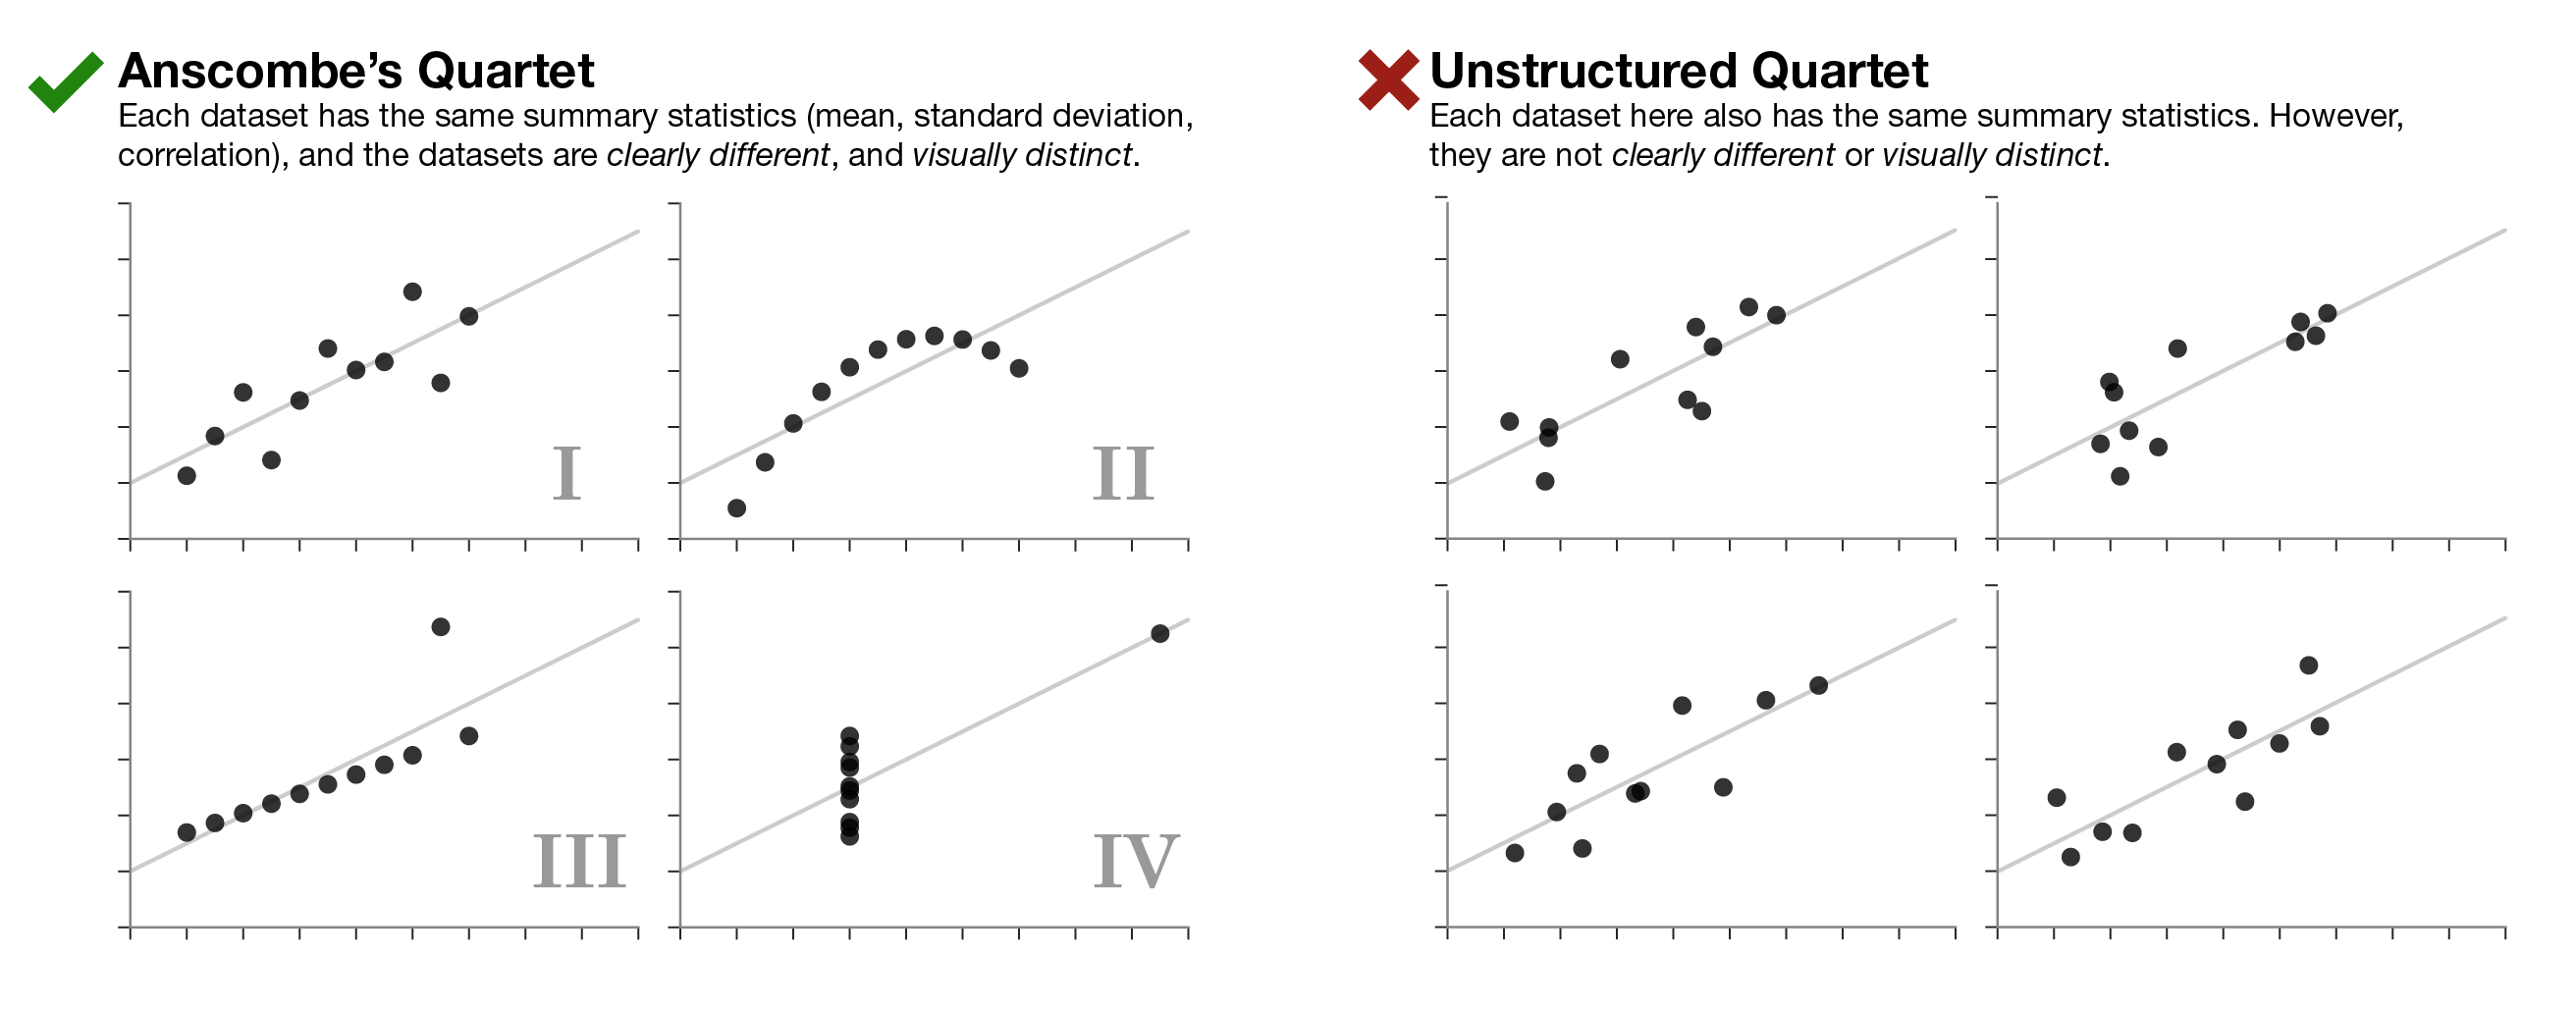
\includegraphics[width=\linewidth]{images/anscombe-quartet-comparison.png}
    \caption{Anscombe's Quartet (left) compared with an unstructured quartet (right): both can share summary statistics, but only the left side is clearly visually distinct \parencite{anscombe1973, matejka2017}.}
    \label{fig:anscombe-quartet}
\end{figure*}
Figure~\ref{fig:anscombe-quartet} makes the mismatch explicit. Dataset I is roughly linear with moderate noise, Dataset II shows curvature, Dataset III is dominated by an outlier, and Dataset IV concentrates points at one x-value with a high-leverage point. The same summary statistic values therefore do not imply the same analytical story.

This lesson generalises directly: \textit{important structure can be hidden in summary metrics}. For this reason, statistical analysis should be paired with visual inspection before final conclusions. The ``Same Stats, Different Graphs'' work by J. Matejka and G. Fitzmaurice gives a strong demonstration (See Figure~\ref{fig:datasaurus-dozen}).

\begin{figure*}[tbp]
    \centering
    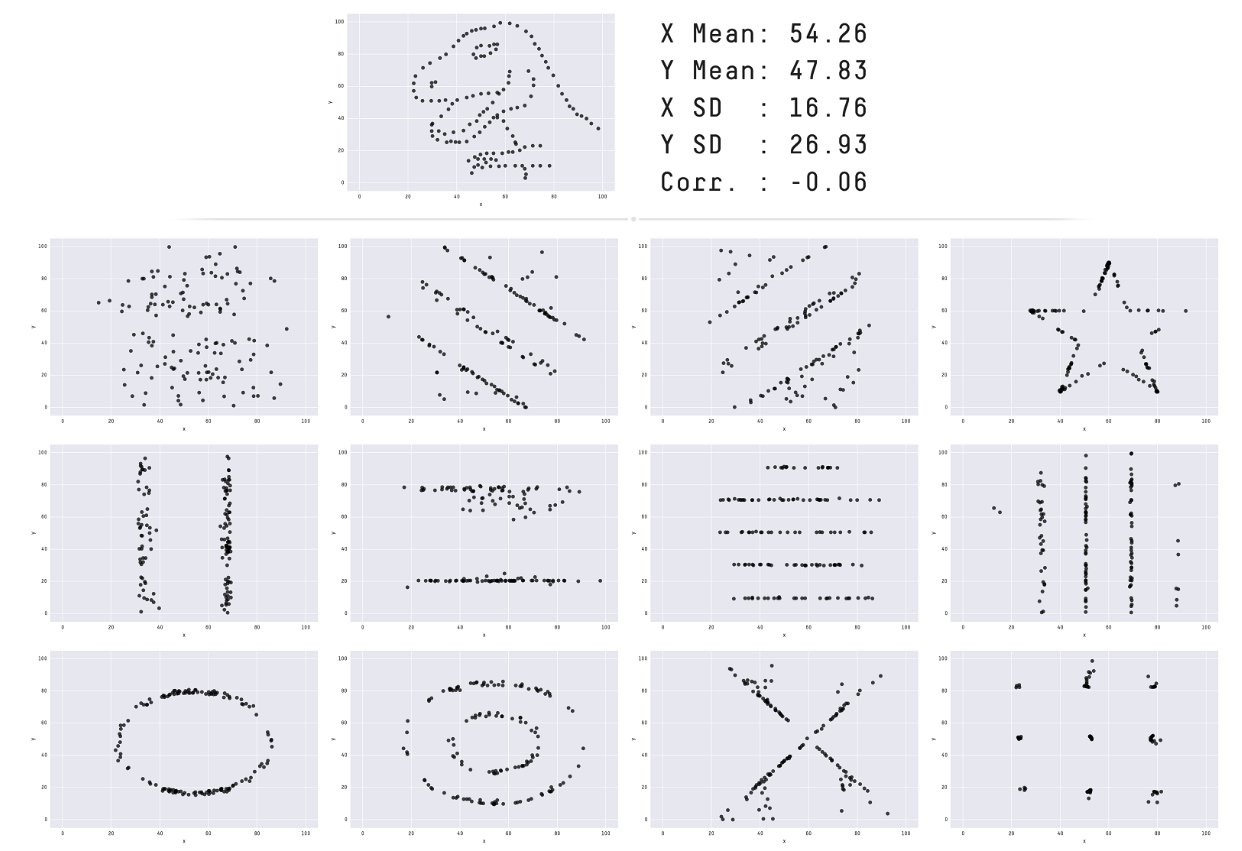
\includegraphics[width=\linewidth]{images/same_stats_different_graphs_dinosaur.png}
    \caption{The Datasaurus Dozen: datasets with very different shapes but matching summary statistics (mean, standard deviation, and Pearson correlation) to two decimal places. This shows why visual inspection is essential in analysis and communication \parencite{matejka2017}.}
    \label{fig:datasaurus-dozen}
\end{figure*}

\section{Practical Workflow and Limits}

Visualisation design follows an iterative workflow: \textbf{collect data}, \textbf{assess data quality}, \textbf{choose/design an idiom}, \textbf{evaluate and refine} (including clutter control, aesthetics, and effectiveness), and \textbf{communicate}. The steps are not linear; revisions are expected whenever new issues appear.

It also highlights practical limits. Very large datasets can exceed compute or rendering capacity; screen space is finite; and human perception is powerful but imperfect. In real projects, we often trade off between showing more data and preserving readability.
\marginnotebox{LIMITS NOTE}{Three practical constraints:\par \textbullet\ \textbf{Computer limits} (especially interactive performance)\par \textbullet\ \textbf{Human limits} (perceptual and cognitive)\par \textbullet\ \textbf{Display limits} (finite pixels)\par Design always trades off data density against clutter.\par Examples: \href{https://en.wikipedia.org/wiki/Misleading_graph}{Wikipedia: Misleading graph}; \href{http://www.abc.net.au/news/2013-05-08/iericho-read-between-the-lines/4674322}{ABC News: Read between the lines}.}

\section{Analysis Framework: Four Levels and Three Questions}
\label{sec:analysis-framework}

Once we know why visual inspection matters, we need a systematic method for design and critique. Munzner proposes four levels of design: (1) domain situation, (2) data/task abstraction, (3) visual encoding and interaction, and (4) algorithm \parencite{munzner2014}. Across these levels, we repeatedly ask three linked questions: \textit{why} is the task performed, \textit{what} data is involved, and \textit{how} should the visualisation encode and support interaction.

\begin{marginfigure}[-10\baselineskip]
    \centering
    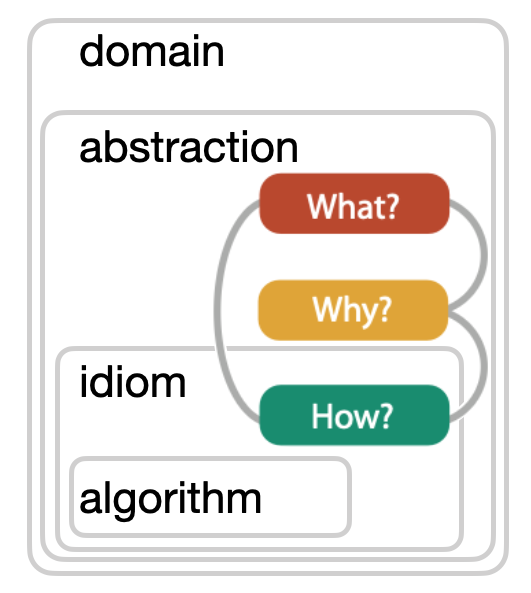
\includegraphics[width=0.9\linewidth]{images/what-why-how.png}
    \caption{Relationship between the four levels (domain, abstraction, idiom, algorithm) and the three questions (What, Why, How) \parencite{munzner2014}.}
    \label{fig:what-why-how-margin}
\end{marginfigure}


Figure~\ref{fig:what-why-how-margin} and Table~\ref{tab:three-questions-four-levels} present complementary perspectives on the same relationship: \textit{What} and \textit{Why} are addressed primarily at the abstraction level, \textit{How} at the idiom level, while algorithms realise the idiom within domain constraints. Used together, the figure conveys the conceptual nesting, and the table specifies the explicit mapping adopted in this unit.

\begin{table*}[tbp]
    \centering
    \small
    \begin{tabular}{@{}p{0.22\linewidth}p{0.36\linewidth}p{0.38\linewidth}@{}}
        \textbf{The 3 Questions} & \textbf{The 4 Levels (Nested Model)} & \textbf{Focus} \\
        \hline
        \textit{(Context)} & \textbf{1. Domain Situation} & Who are the users? \\
        \textbf{What?} & \textbf{2. Data \& Task Abstraction} & What data is used? \\
        \textbf{Why?} & \textbf{2. Data \& Task Abstraction} & What is the goal? \\
        \textbf{How?} & \textbf{3. Idiom} & Visual design choices. \\
        \textit{(Implementation)} & \textbf{4. Algorithm} & Efficient computer code. \\
    \end{tabular}
    \caption{Summary mapping between the Three Questions and the Four Levels (Nested Model) \parencite{munzner2014}.}
    \label{tab:three-questions-four-levels}
\end{table*}


\subsection*{1) Domain situation}
The first level identifies the domain context: who the users are, what domain-specific language they use, and which constraints shape their workflow. Without this grounding, later design choices may be technically correct but practically irrelevant. In a representative example, the domain is urban public transport planning and the user is a punctuality analyst.

\subsection*{2) Data and task abstraction (What and Why)}
At this level, we translate domain language into abstract data and task language. In practice, this means clarifying \textit{what} data structures are present and \textit{why} users need to inspect them.~\sidenote{For example, train stations and tracks become nodes and links; the goal (why) may be understanding travel-time access to stops. Once these points are explicit, later encoding decisions become easier to justify and evaluate.}

\subsection*{3) Visual encoding and interaction (How)}
The third level turns abstraction into a visual idiom. At this stage, we choose marks, channels, layouts, and interactions that directly support the goals identified at the previous level.

\subsection*{4) Algorithm}
The fourth level concerns implementation. Here, we focus on the algorithms and engineering choices needed to deliver the chosen idiom at useful speed and scale.

\setsectionaccent{whataccent}
\section{Data Abstraction (The ``What'')}
\label{sec:what-why-how}
\label{sec:data-abstraction}
With the framework in place, we now unpack the three guiding questions one by one. We start with \textit{what}: the structure and meaning of the data.
\marginnotebox{WHAT NOTE}{For more detail on \textbf{What}, see \textbf{Topic: Data Types}.}

Data abstraction describes data structure and meaning independently of domain details. It helps us choose suitable encodings and avoid misleading designs.

\begin{figure*}
    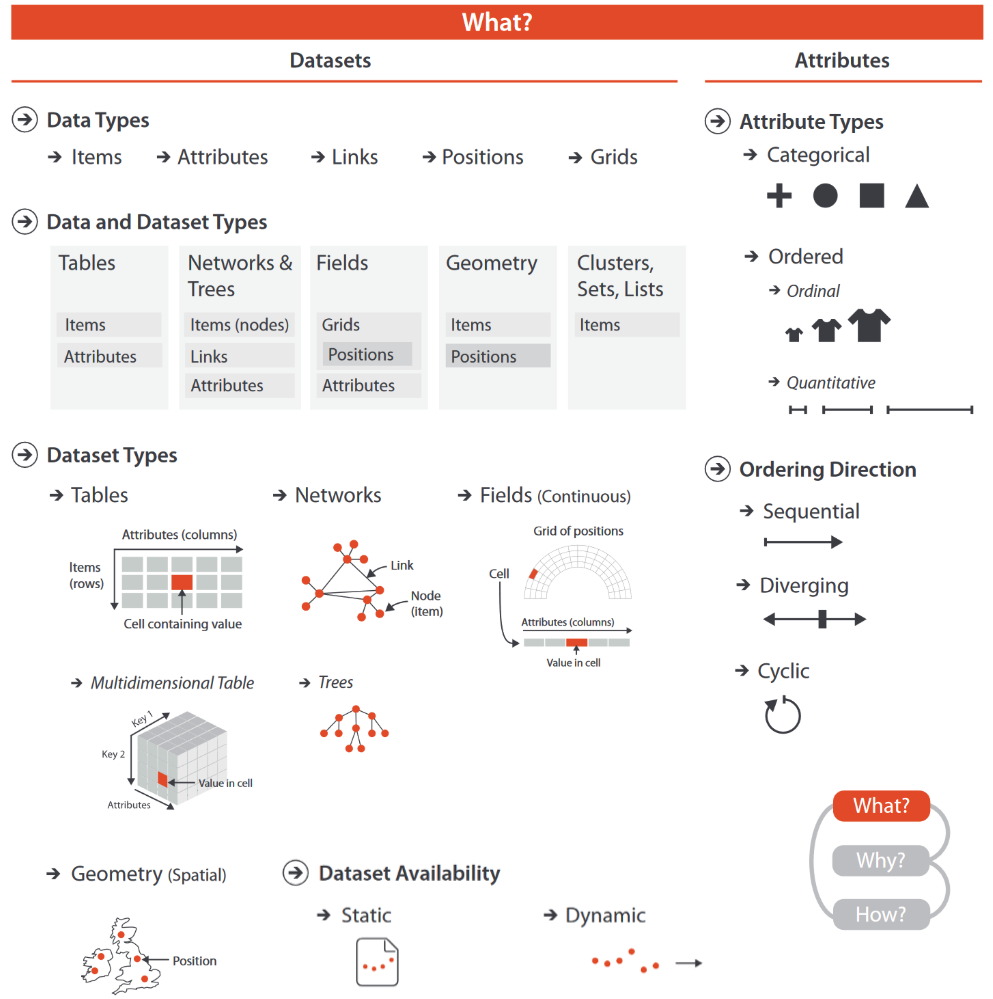
\includegraphics[width=0.9\linewidth]{images/what.png}
    \caption{Munzner's \textit{what} abstraction space: classify \textbf{dataset structure} first, then classify \textbf{attribute type and semantics}, before choosing any encoding \parencite{munzner2014}.}
    \label{fig:what-abstraction}
\end{figure*}
Figure~\ref{fig:what-abstraction} should be read in two passes. First identify dataset structure (such as table, network, field, or geometry), because structure determines valid operations and layouts. Then classify attributes (categorical vs ordered; key vs value), because attribute semantics determine which channels can encode values correctly \parencite{munzner2014}.

\subsection*{Data and dataset types}
At the lowest level, we describe data using \textbf{items}, \textbf{attributes}, \textbf{links}, \textbf{positions}, and \textbf{grids}. Items are the entities we analyse, attributes are their properties, and links describe relationships between items. Positions and grids become important when the data is spatial or sampled from continuous space.

These building blocks combine into familiar dataset forms. \textbf{Tables} organise rows and columns; \textbf{networks (graphs)} organise nodes and links; \textbf{fields}~\sidenote{Observed samples from an underlying continuous phenomenon.} sample values across space, often as scalar, vector, or tensor quantities; and \textbf{geometry} carries explicit shape and location. This classification helps prevent mismatches between data structure and chart form.

A key operational difference is that tables can usually be reordered (for example, sort rows) without changing meaning, while spatial fields cannot be arbitrarily reordered because position is part of the data semantics.

\marginnotebox{%
\textbf{Common Vocabulary}\par
\textbullet\ \textbf{Network} = graph\par
\textbullet\ \textbf{Node} = vertex\par
\textbullet\ \textbf{Link} = edge\par
}

\subsection*{Attribute types}
Attribute meaning is the second part of abstraction. \textbf{Categorical (nominal)} attributes encode identity without order, while \textbf{ordered} attributes encode rank or magnitude. Ordered attributes may be \textit{ordinal}, where rank matters but distance does not, or \textit{quantitative}, where arithmetic comparisons are valid. Direction then refines interpretation: values can be \textit{sequential}, \textit{diverging}, or \textit{cyclic}~\sidenote{Typical examples: beach visits in a year are \textit{sequential}, elevation above/below sea level is \textit{diverging}, and weekday or month patterns are \textit{cyclic}.}.

\textbf{Semantics.} Finally, we separate \textbf{keys} and \textbf{values}. Keys identify items and support lookup, while values store measured or derived quantities to compare.

\setsectionaccent{whyaccent}
\section{Task Abstraction (The ``Why'')}
\label{sec:task-abstraction}

\begin{figure*}[tbp]
    \centering
    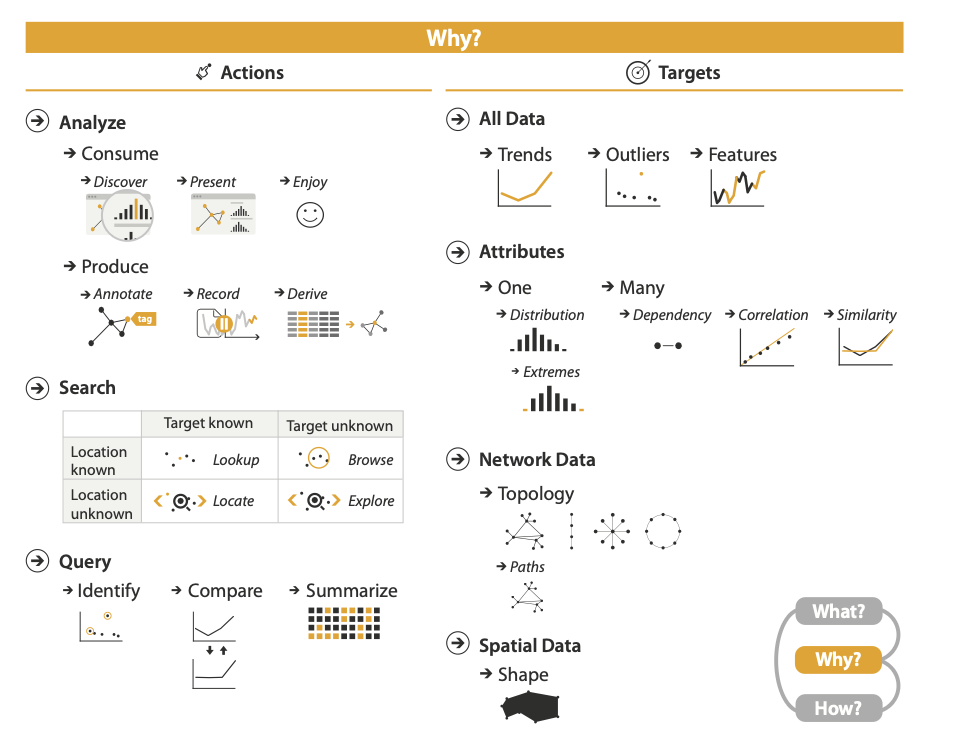
\includegraphics[width=\linewidth]{images/why.png}
    \caption{Munzner's \textit{why} abstraction space: tasks are specified as \textbf{actions} applied to \textbf{targets} \parencite{munzner2014}.}
    \label{fig:why-abstraction}
\end{figure*}


In this unit, \textit{why} follows Munzner's task abstraction: goals are specified as \textbf{actions} applied to \textbf{targets}. Typical goals include identifying \textbf{correlation}, comparing \textbf{similarity}, understanding \textbf{distribution}, detecting \textbf{trends over time}, finding \textbf{outliers}, and recognising notable \textbf{features}.

In this \textbf{actions-and-targets} view, actions include \textbf{analyse} (consume, produce), \textbf{search}, and \textbf{query}; targets include all data, subsets, or individual attributes/relationships.
\marginnotebox{NOTE}{This section starts with Munzner's \textbf{action-target} \textbf{Why} model (Figure~\ref{fig:why-abstraction}). For extended explanatory \textbf{Why} design, see \textbf{Topic: How to Tell a Story with Data Visualisation}.}

Figure~\ref{fig:why-abstraction} is read by combining one action family with one target type. On the action side, analysts may \textbf{analyse} (consume/produce), \textbf{search} (lookup, locate, browse, explore), or \textbf{query} (identify, compare, summarise). On the target side, tasks may concern all data, attribute relationships, network structure, or spatial structure. A specific task is therefore an action-target pair, such as \textbf{compare} + \textbf{attributes} or \textbf{explore} + \textbf{all data} \parencite{munzner2014}.

In the \textbf{consume} branch, common intents are \textbf{discover} and \textbf{enjoy}; in the \textbf{produce} branch, common actions are \textbf{annotate}, \textbf{record}, \textbf{derive}, and \textbf{present}. \textbf{Derive is especially important}: task-relevant transformed attributes are often easier to interpret than raw ones.

\subsection*{From Action-Target to Function–Form}
\margincitebox[Form vs Function]{schwabish2021}

We map Munzner's action-target \textit{why} space to a \textbf{function} continuum: \textbf{Exploration $\rightarrow$ Explanation}.

\begin{marginfigure}
    \centering
    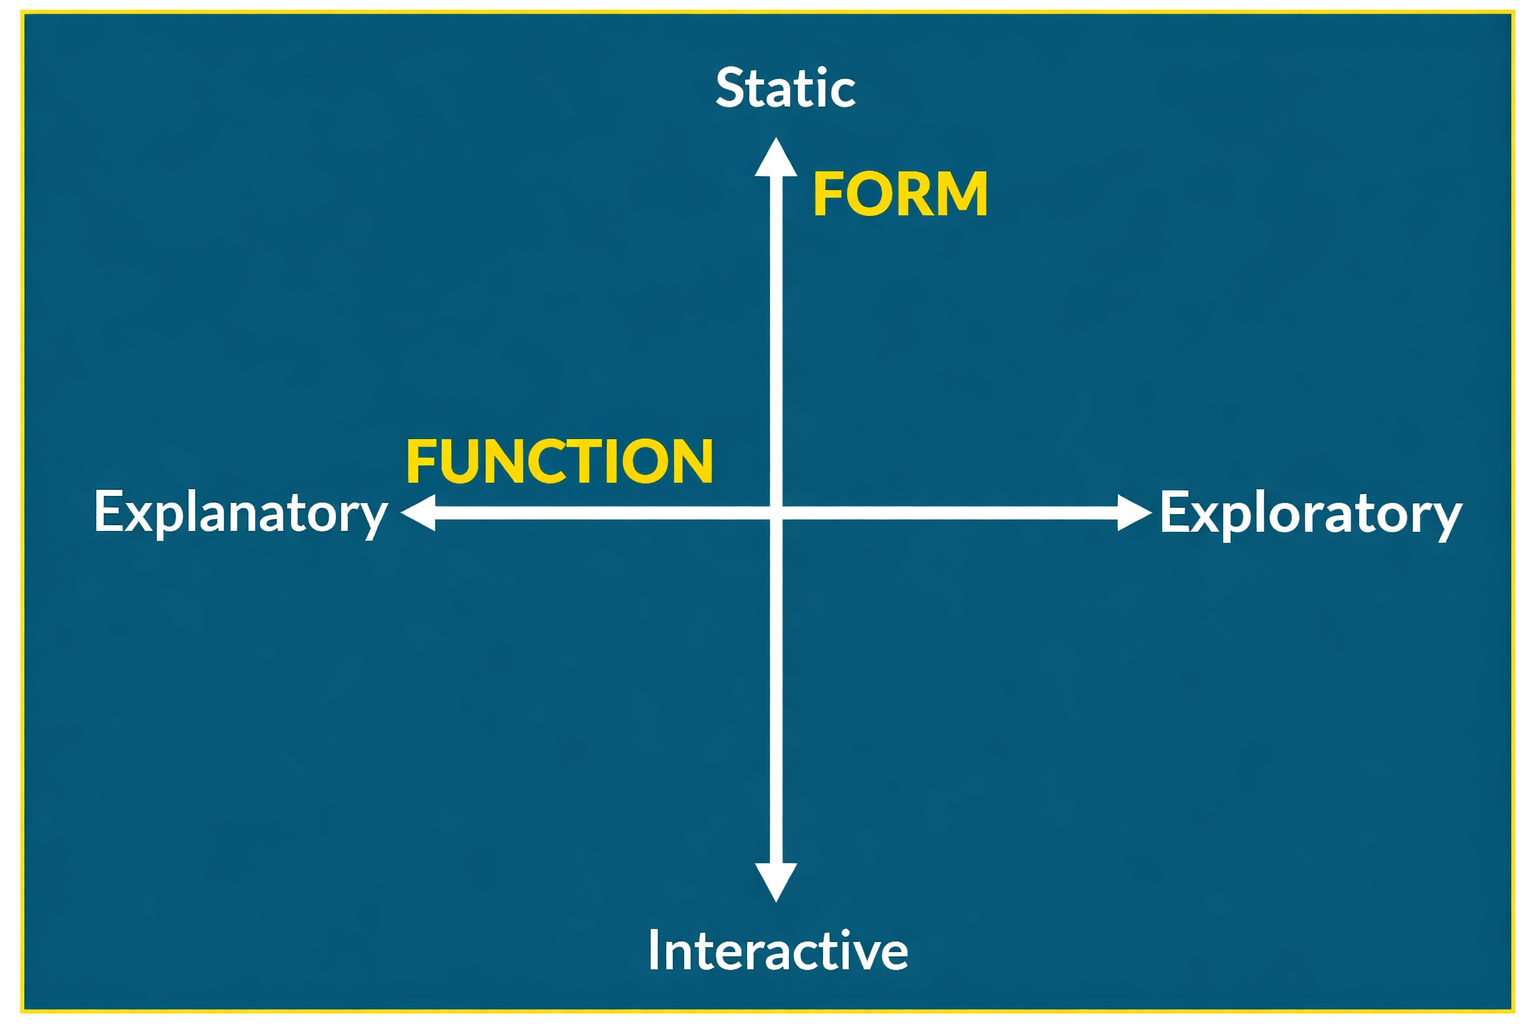
\includegraphics[width=\linewidth]{images/form-function-intro.png}
    \caption{Function–Form Quadrant of Data Visualisation: \textbf{x-axis} is \textbf{function} (exploratory--explanatory, \textit{why}); \textbf{y-axis} is \textbf{form} (static--interactive, mainly \textit{how}).}
    \label{fig:form-function-intro}
\end{marginfigure}


In Munzner's full \textit{why} taxonomy, \textbf{exploration} aligns mainly with \textbf{Analyze $\rightarrow$ Consume $\rightarrow$ Discover}, plus substantial \textbf{Search} (especially target/location unknown cases such as browse and explore) and \textbf{Query} (identify, compare, summarise). Exploration often includes \textbf{Produce} actions such as \textbf{Derive} and \textbf{Annotate} as intermediate analysis artefacts. \textbf{Explanation} aligns mainly with \textbf{Present}: communicating conclusions to an audience with clearer targets and more controlled paths.

In this unit, this mapping is a deliberate simplification of Munzner's richer action-target space. It clarifies scope: we retain the core \textit{why} logic, but treat it as a progression from open-ended analysis to directed communication.

After discussing \textbf{function} (\textit{why}) on the x-axis, we turn to \textbf{form} on the y-axis: \textbf{static $\leftrightarrow$ interactive}. This is the \textit{how} side of Figure~\ref{fig:form-function-intro}. The two axes are related in practice but conceptually distinct.


\setsectionaccent{howaccent}
\section{Marks and Channels (The ``How'')}
\label{sec:marks-channels}
With \textit{what} and \textit{why} defined, we can now decide \textit{how} to encode the data. Visual encoding maps abstract data to perceivable form. Good encodings make important patterns easy to see and hard to misread.
\marginnotebox{HOW NOTE}{For more detail on \textbf{How}, see \textbf{Topic: Marks and Channels}.}

In this unit, \textbf{marks and channels} correspond roughly to the \textbf{static} part of Munzner's \textit{how} space, mainly the \textbf{Encode} branch (map/express). The full \textit{how} scope is broader: it also includes the \textbf{interactive} parts---\textbf{Manipulate} (interaction changes such as select, navigate, change), \textbf{Facet} (multi-view composition such as juxtapose, partition, superimpose), \textbf{Reduce} (filtering and aggregation), and \textbf{Embed} (focus+context). These interactive \textit{how} components are introduced for context, but detailed mastery is \textbf{not required} in this unit.

\begin{figure*}
    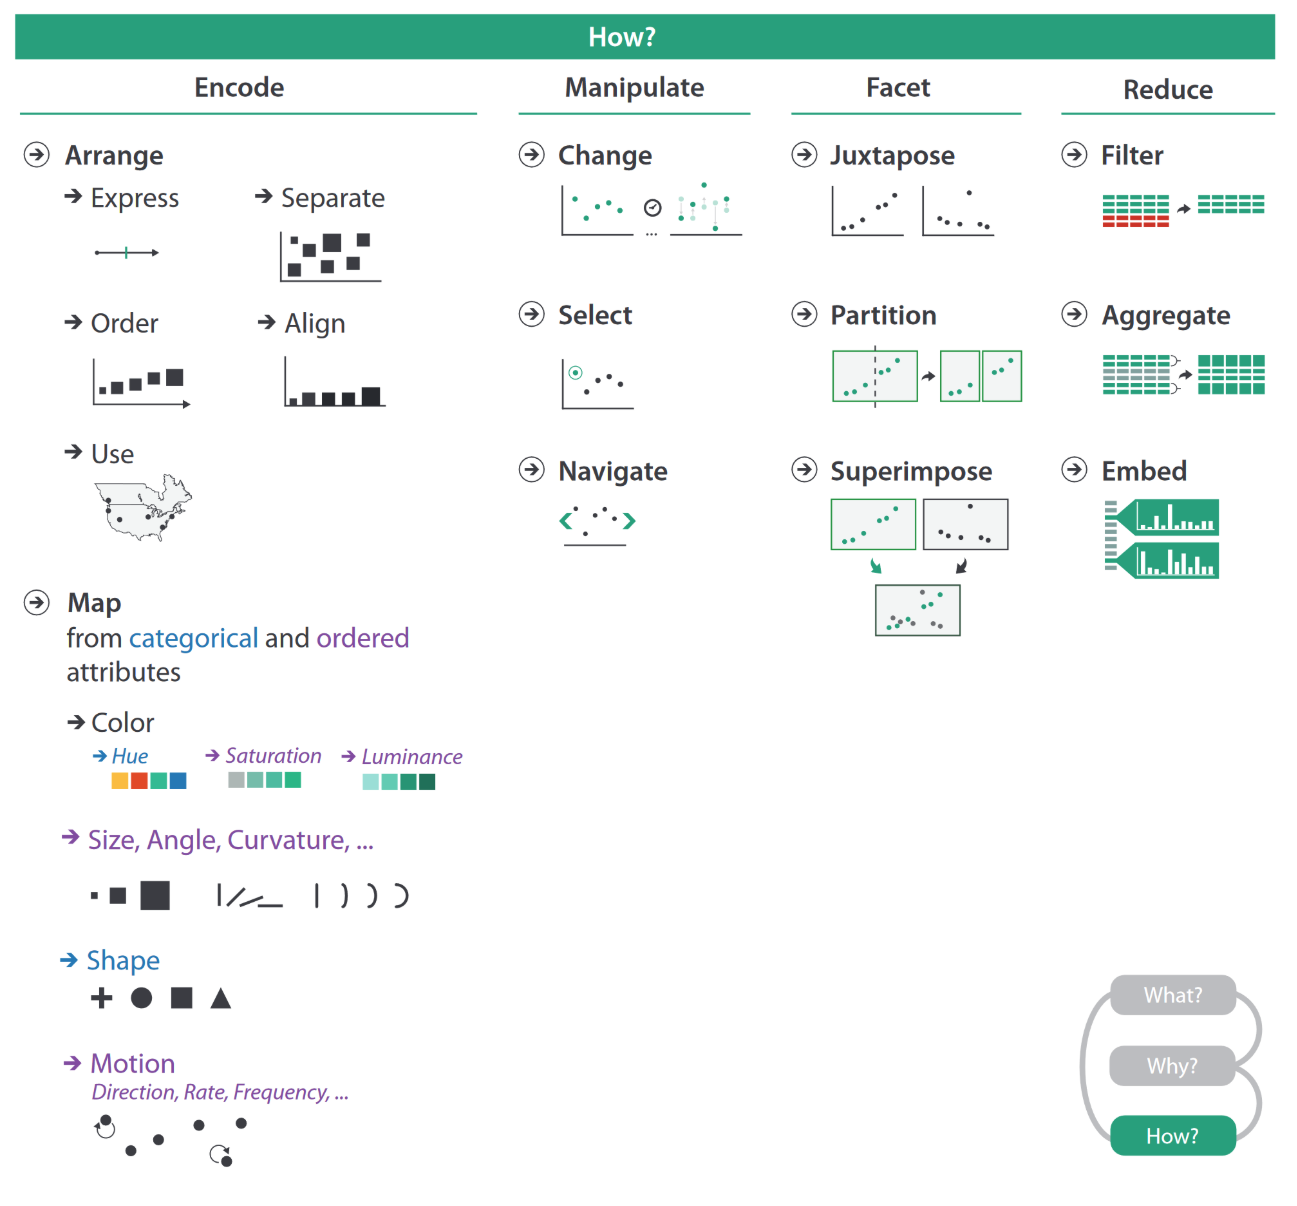
\includegraphics[width=\linewidth]{images/how.png}
    \caption{Munzner's \textit{how} design space: \textbf{Encode}, \textbf{Manipulate}, \textbf{Facet}, and \textbf{Reduce}. In this unit, required mastery is the static \textbf{Encode} branch, with other branches introduced as context \parencite{munzner2014}.}
    \label{fig:how-encoding}
\end{figure*}
Figure~\ref{fig:how-encoding} clarifies that \textit{how} is broader than a chart type. \textbf{Encode} selects marks and channels; \textbf{Manipulate} supports interaction changes; \textbf{Facet} organises multi-view composition; and \textbf{Reduce} controls scale through filtering or aggregation. In this topic, we go deepest on \textbf{Encode} so that encoding decisions remain consistent with the previously defined \textit{what} and \textit{why} \parencite{munzner2014}.

\subsection*{Encode}
\textbf{Marks} are geometric primitives that represent items and links, and the most common mark types are \textit{points} (0D), \textit{lines} (1D), and \textit{areas} (2D). In practice, lines often communicate \textit{connection} and areas often communicate \textit{containment}. A key reminder is that a mark specifies geometry, not appearance. \textbf{Channels} control appearance and carry data meaning through properties such as position, size, shape, orientation, colour, and motion.

For colour, the three channels are \textbf{hue} (which pure colour), \textbf{luminance/value} (light vs dark), and \textbf{saturation} (gray vs pure colour).

\begin{figure*}[tbp]
    \centering
    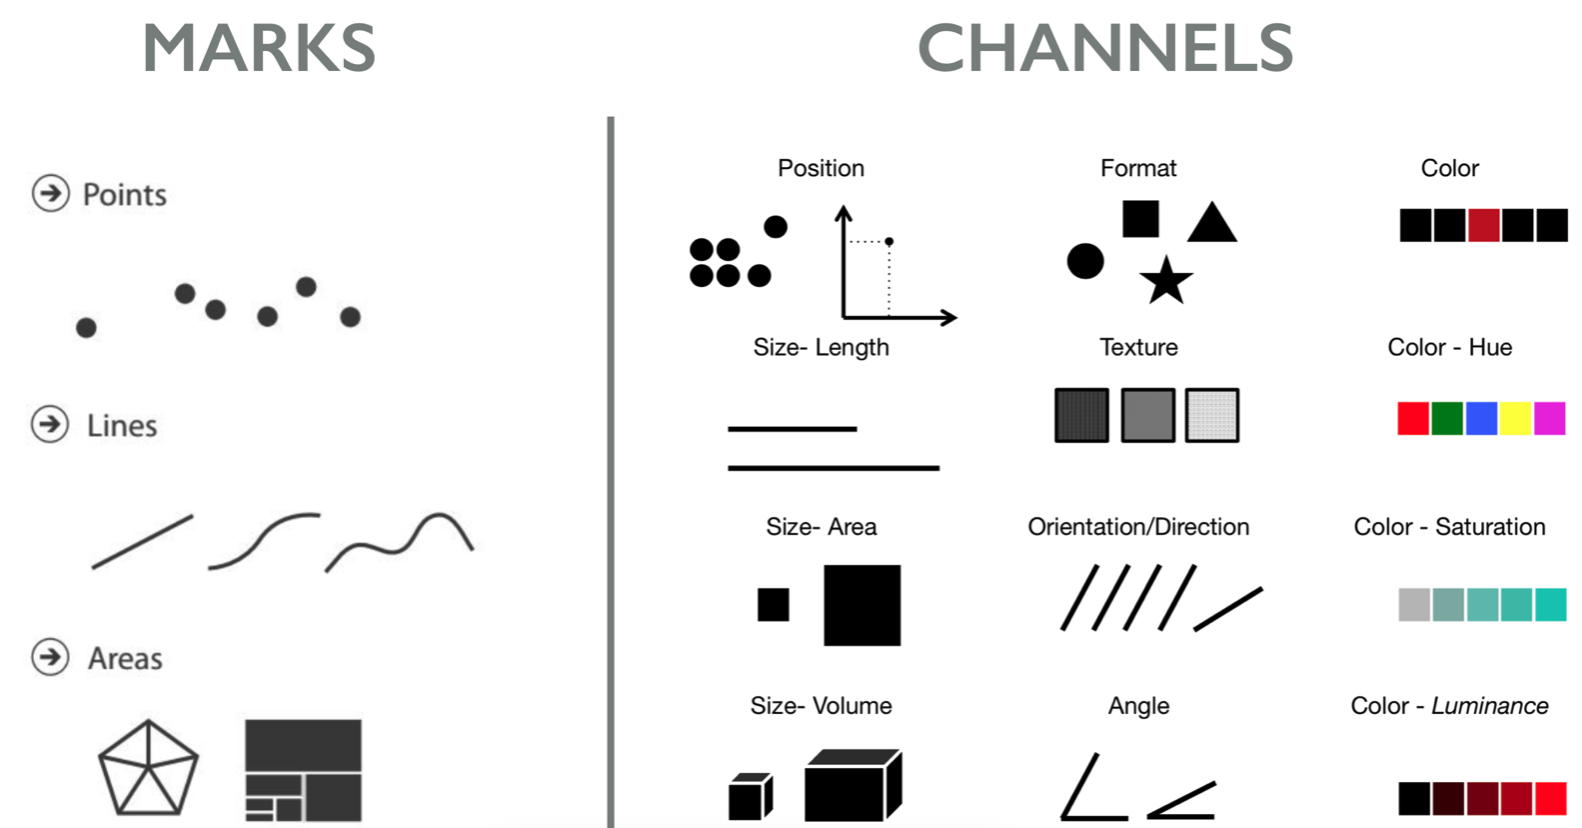
\includegraphics[width=\linewidth]{images/marks-channels.png}
    \caption{Static encoding focus for this unit: marks and channels matrix showing which channels are available for points, lines, and areas, and how suitability differs for ordered versus categorical attributes \parencite{munzner2014}.}
    \label{fig:marks-channels-matrix}
\end{figure*}
Figure~\ref{fig:marks-channels-matrix} is the practical lookup used in this topic: first choose a mark family, then choose channels that match the attribute type and task.

\subsection*{Redundant and Multivariate Encoding}
\textbf{Redundant encoding} means using multiple channels to represent the same attribute (e.g., both colour and shape for category), which can improve robustness and readability, especially if one channel is hard to perceive. \textbf{Multivariate encoding} means using different channels to encode different attributes, allowing more information to be shown at once. Both strategies should be used deliberately, based on task needs and perceptual limits.

\marginnotebox{CORE PRINCIPLES}{Two principles guide these decisions. \textbf{Expressiveness} means the encoding should represent all and only the intended information, while \textbf{effectiveness} means the most important attributes should be mapped to the channels people can judge most accurately.}

\subsection*{Channel effectiveness rankings}
For \textbf{ordered data} (``how much?''), effectiveness generally follows this pattern: \textbf{position on a common scale} is strongest, followed by length, then angle/orientation and area, while volume and colour-based magnitude judgements (luminance/saturation) are usually weakest for precise reading. For \textbf{categorical data} (``what/where?''), spatial region and colour hue are usually strong choices, with shape also useful for identity.

\begin{figure*}[htp]
    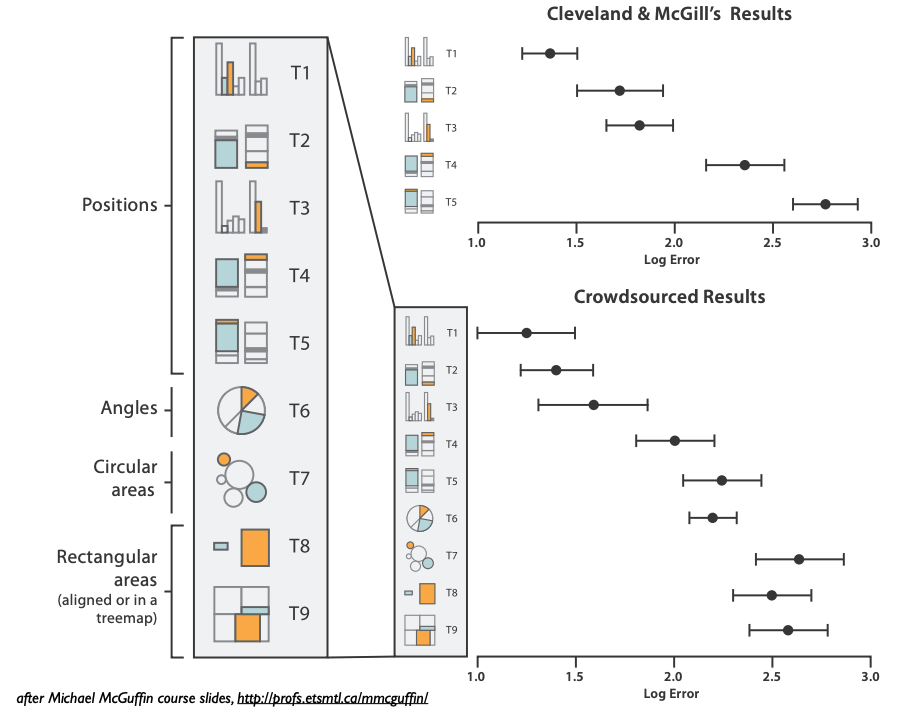
\includegraphics[width=\linewidth]{images/cleveland-mcgill.png}
    \caption{Graphical perception results. Left: ranked task types by channel. Right: log error in Cleveland \& McGill and in Heer \& Bostock's crowdsourced replication \parencite{heer2010}.}
    \label{fig:cleveland-mcgill}
\end{figure*}
Figure~\ref{fig:cleveland-mcgill} grounds the ranking list empirically: channels tied to position and length yield lower estimation error than area, volume, and colour-based magnitude judgements.

\margincitebox{heer2010}

\section{Example: Gapminder Bubble Chart}

To make the framework concrete, we use the Gapminder bubble chart (life expectancy vs GDP per capita over time) as a worked example \parencite{gapmindertools}.

\begin{figure}[htbp]
    \centering
    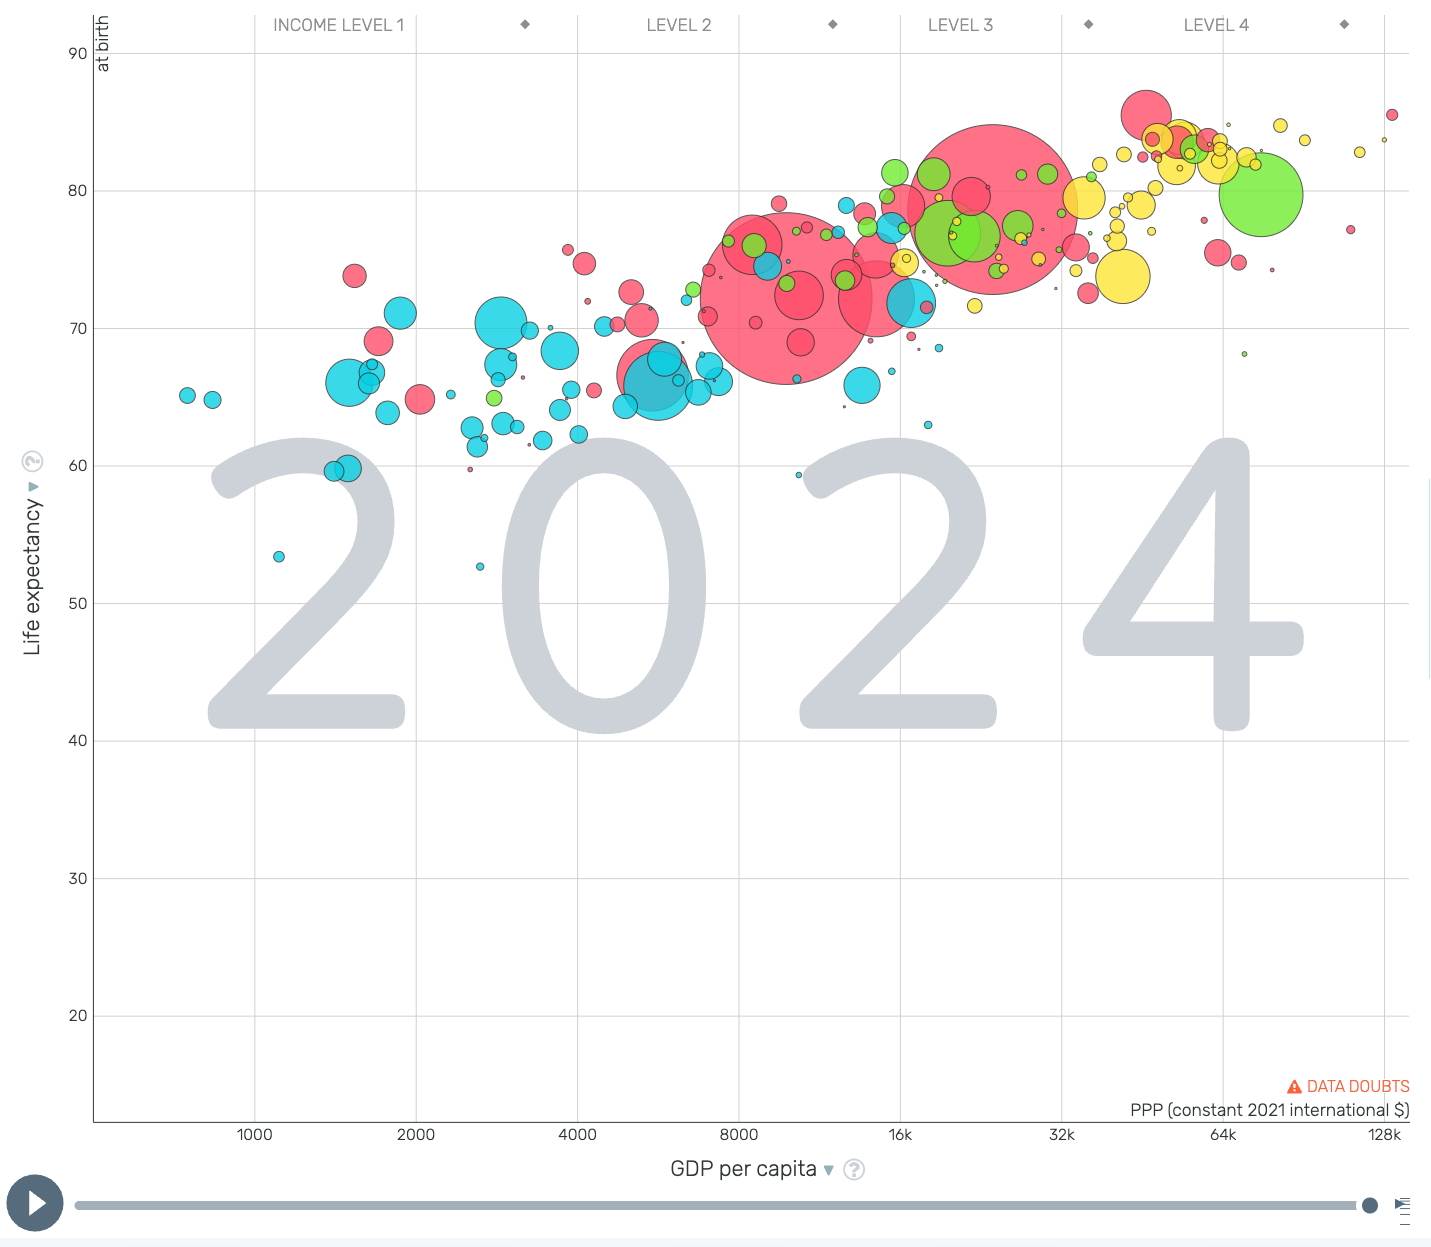
\includegraphics[width=\textwidth]{images/gapminder-life-expectancy-vs-gdp-per-capita.png}
    \caption{Gapminder bubble chart example used to explain \textit{what}--\textit{why}--\textit{how} \parencite{gapmindertools}.}
    \label{fig:gapminder-example}
\end{figure}

\margincitebox[The Gapminder Example]{gapmindertools}

\textit{What}: The dataset contains country-level observations of life expectancy, GDP per capita, population, world region, and year. The main \textbf{items} are countries observed over time. Key \textbf{attributes} are GDP per capita and life expectancy (\textbf{quantitative}), population (\textbf{quantitative}), world region (\textbf{categorical}), and year (\textbf{ordered} temporal). This makes the dataset suitable for comparing cross-country differences and temporal change.

\textit{Why}: The main goal is to understand long-run development patterns across countries. In \textbf{actions-and-targets} terms, viewers \textbf{query} to compare countries, \textbf{search} for outliers, and \textbf{analyse} trajectories through time. In \textbf{function} terms, the same chart supports \textbf{Exploration} (open-ended inspection and hypothesis building) and \textbf{Explanation} (communicating long-run development patterns to a broader audience).

\textit{How}: The \textbf{idiom} is an animated bubble scatterplot with circle \textbf{marks}. Primary \textbf{channels} are x-position for GDP per capita, y-position for life expectancy, \textbf{size} for population, and \textbf{colour hue} for world region; time is shown with motion along the timeline. In \textbf{form} terms, interaction (play/pause, scrubbing, hover/filter) supports exploratory reading, while static snapshots can support explanatory communication.

This example shows the full design chain in order: define \textit{what} data exists, specify \textit{why} tasks and \textbf{function}, then choose \textit{how} through \textbf{form}, \textbf{marks}, and \textbf{channels}. Using this sequence helps keep visual decisions aligned with analytical goals instead of chart style alone.
